%package list
\documentclass{article}
\usepackage[top=3cm, bottom=3cm, outer=3cm, inner=3cm]{geometry}
\usepackage{multicol}
\usepackage{graphicx}
\usepackage{caption} % Opcional, para personalizar las leyendas
\usepackage{subcaption} % Opcional, para organizar imágenes en subfiguras
\usepackage{url}
%\usepackage{cite}
\usepackage{hyperref}
\usepackage{array}
%\usepackage{multicol}
\newcolumntype{x}[1]{>{\centering\arraybackslash\hspace{0pt}}p{#1}}
\usepackage{natbib}
\usepackage{pdfpages}
\usepackage{multirow}
\usepackage[normalem]{ulem}
\useunder{\uline}{\ul}{}
\usepackage{svg}
\usepackage{xcolor}
\usepackage{listings}
\lstdefinestyle{ascii-tree}{
    literate={├}{|}1 {─}{--}1 {└}{+}1 
  }
\lstset{basicstyle=\ttfamily,
  showstringspaces=false,
  commentstyle=\color{red},
  keywordstyle=\color{blue}
}
%\usepackage{booktabs}
\usepackage{caption}
\usepackage{subcaption}
\usepackage{float}
\usepackage{array}

\newcolumntype{M}[1]{>{\centering\arraybackslash}m{#1}}
\newcolumntype{N}{@{}m{0pt}@{}}


%%%%%%%%%%%%%%%%%%%%%%%%%%%%%%%%%%%%%%%%%%%%%%%%%%%%%%%%%%%%%%%%%%%%%%%%%%%%
%%%%%%%%%%%%%%%%%%%%%%%%%%%%%%%%%%%%%%%%%%%%%%%%%%%%%%%%%%%%%%%%%%%%%%%%%%%%
\newcommand{\itemCourse}{Programación Web I}
\newcommand{\itemSemester}{II}
\newcommand{\itemUniversity}{Universidad Nacional de San Agustín de Arequipa}
\newcommand{\itemFaculty}{Facultad de Ingeniería de Producción y Servicios}
\newcommand{\itemDepartment}{Departamento Académico de Ingeniería de Sistemas e Informática}
\newcommand{\itemSchool}{Escuela Profesional de Ingeniería de Sistemas}
\newcommand{\itemAcademic}{2024 - B}
\newcommand{\itemInput}{Del 12 Noviembre 2024}
\newcommand{\itemOutput}{Al 17 Noviembre 2024}
\newcommand{\itemPracticeNumber}{06}
\newcommand{\itemTheme}{Git y GitHub}
%%%%%%%%%%%%%%%%%%%%%%%%%%%%%%%%%%%%%%%%%%%%%%%%%%%%%%%%%%%%%%%%%%%%%%%%%%%%
%%%%%%%%%%%%%%%%%%%%%%%%%%%%%%%%%%%%%%%%%%%%%%%%%%%%%%%%%%%%%%%%%%%%%%%%%%%%

\usepackage[english,spanish]{babel}
\usepackage[utf8]{inputenc}
\AtBeginDocument{\selectlanguage{spanish}}
\renewcommand{\figurename}{Figura}
\renewcommand{\refname}{Referencias}
\renewcommand{\tablename}{Tabla} %esto no funciona cuando se usa babel
\AtBeginDocument{%
	\renewcommand\tablename{Tabla}
}

\usepackage{fancyhdr}
\pagestyle{fancy}
\fancyhf{}
\setlength{\headheight}{30pt}
\renewcommand{\headrulewidth}{1pt}
\renewcommand{\footrulewidth}{1pt}
\fancyhead[L]{\raisebox{-0.2\height}{\includegraphics[width=3cm]{img/logo_episunsa.png}}}
\fancyhead[C]{\fontsize{7}{7}\selectfont	\itemUniversity \\ \itemFaculty \\ \itemDepartment \\ \itemSchool \\ \textbf{\itemCourse}}
\fancyhead[R]{\raisebox{-0.2\height}{\includegraphics[width=1.2cm]{img/logo_abet}}}
\fancyfoot[L]{Ingeniería de Sistemas}
\fancyfoot[C]{\itemCourse}
\fancyfoot[R]{Página \thepage}

% para el codigo fuente
\usepackage{listings}
\usepackage{color, colortbl}
\definecolor{dkgreen}{rgb}{0,0.6,0}
\definecolor{gray}{rgb}{0.5,0.5,0.5}
\definecolor{mauve}{rgb}{0.58,0,0.82}
\definecolor{codebackground}{rgb}{0.95, 0.95, 0.92}
\definecolor{tablebackground}{rgb}{0.8, 0, 0}

\lstset{frame=tb,
	language=bash,
	aboveskip=3mm,
	belowskip=3mm,
	showstringspaces=false,
	columns=flexible,
	basicstyle={\small\ttfamily},
	numbers=none,
	numberstyle=\tiny\color{gray},
	keywordstyle=\color{blue},
	commentstyle=\color{dkgreen},
	stringstyle=\color{mauve},
	breaklines=true,
	breakatwhitespace=true,
	tabsize=3,
	backgroundcolor= \color{codebackground},
}

\begin{document}
	
	\vspace*{10px}
	
	\begin{center}	
		\fontsize{17}{17} \textbf{ Informe de Laboratorio \itemPracticeNumber}
	\end{center}
	\centerline{\textbf{\Large Tema: \itemTheme}}
	%\vspace*{0.5cm}	

	\begin{flushright}
		\begin{tabular}{|M{2.5cm}|N|}
			\hline 
			\rowcolor{tablebackground}
			\color{white} \textbf{Nota}  \\
			\hline 
			     \\[30pt]
			\hline 			
		\end{tabular}
	\end{flushright}	

    \begin{table}[H]
    	\begin{tabular}{|x{4.7cm}|x{4.8cm}|x{4.8cm}|}
    		\hline 
    		\rowcolor{tablebackground}
    		\color{white} \textbf{Estudiante} & \color{white}\textbf{Escuela}  & \color{white}\textbf{Asignatura}   \\
    		\hline 
    		{Auccacusi Conde Brayan Carlos \par bauccacusic@unsa.edu.pe} & \itemSchool & {\itemCourse \par Semestre: \itemSemester \par Código: 20211196}     \\
    		\hline 
    		{Palma Apaza Santiago Enrique \par spalmaa@unsa.edu.pe} & \itemSchool & {\itemCourse \par Semestre: \itemSemester \par Código:  20240689}     \\
            \hline 
    		{Pamo Condori Benjamin Andre \par bpamoc@unsa.edu.pe} & \itemSchool & {\itemCourse \par Semestre: \itemSemester \par Código: 20233480}     \\
    		\hline
    		{Huaynacho Mango Jerry Anderson \par jhuaynacho@unsa.edu.pe} & \itemSchool & {\itemCourse \par Semestre: \itemSemester \par Código: 20142322}     \\
    		\hline
    	\end{tabular}
    \end{table}

	
	\begin{table}[H]
		\begin{tabular}{|x{4.7cm}|x{4.8cm}|x{4.8cm}|}
			\hline 
			\rowcolor{tablebackground}
			\color{white}\textbf{Laboratorio} & \color{white}\textbf{Tema}  & \color{white}\textbf{Duración}   \\
			\hline 
			\itemPracticeNumber & \itemTheme & 04 horas   \\
			\hline 
		\end{tabular}
	\end{table}
	
	\begin{table}[H]
		\begin{tabular}{|x{4.7cm}|x{4.8cm}|x{4.8cm}|}
			\hline 
			\rowcolor{tablebackground}
			\color{white}\textbf{Semestre académico} & \color{white}\textbf{Fecha de inicio}  & \color{white}\textbf{Fecha de entrega}   \\
			\hline 
			\itemAcademic & \itemInput &  \itemOutput  \\
			\hline 
		\end{tabular}
	\end{table}
	
    \section{Introducción}
    
    \subsection*{Objetivo del Informe}
    Presentar el desarrollo de una aplicación web que permite realizar consultas dinámicas sobre universidades licenciadas en Perú, utilizando scripts CGI escritos en \textbf{Perl}, \textbf{HTML}, \textbf{CSS} y expresiones regulares. La aplicación fue desplegada y ejecutada en un contenedor \textbf{Docker} y se uso \textbf{GitHub} para trabajar de manera colaborativa.
    
    \subsection*{Importancia del Proyecto}
    \begin{itemize}
        \item Utilización de \textbf{Git} y \textbf{GitHub} para el control de versiones y colaboración en equipo.
        \item Introducción al uso de contenedores para implementar y ejecutar aplicaciones web de manera eficiente.
        \item Aplicación de expresiones regulares para el procesamiento automatizado de datos en un archivo CSV.
    \end{itemize}

    \section{Equipos, Materiales y Temas Utilizados}
    
    \subsection*{Equipos}
    \begin{itemize}
        \item Computadoras con capacidad para ejecutar Docker.
        \item Conexión a Internet.
    \end{itemize}
    
    \subsection*{Materiales}
    \begin{itemize}
        \item \textbf{Archivos de datos proporcionados:}
        \begin{itemize}
            \item \texttt{Data\_Universidades\_LAB06.ods} (ODS)
            \item \texttt{Data\_Universidades\_LAB06.csv} (CSV)
            \item \texttt{Licenciamiento Institucional - Diccionario\_1.pdf} (PDF)
            \item \texttt{Programas de Universidades - Diccionario.pdf} (PDF)
        \end{itemize}
        \item \textbf{Software y herramientas:}
        \begin{itemize}
            \item \textbf{Docker:} Para crear la imagen y ejecutar el contenedor.
            \item \textbf{Git:} Control de versiones local.
            \item \textbf{GitHub:} Repositorio remoto.
            \item \textbf{Perl:} Para la lógica del servidor CGI.
            \item \textbf{HTML y CSS:} Para la interfaz del usuario.
            \item \textbf{Navegador web:} Para pruebas de la aplicación.
    		\item VIM 9.0.
    		\item OpenJDK 64-Bits 17.0.7.
        \end{itemize}
    \end{itemize}
    
    \subsection*{Temas trabajados}
    \begin{itemize}
        \item Uso de Git y GitHub.
        \item Desarrollo y ejecución de contenedores con Docker.
        \item Procesamiento de datos mediante expresiones regulares en Perl.
        \item Desarrollo de interfaces web interactivas con CGI, HTML y CSS.
    \end{itemize}


	\section{URL de Repositorio Github}
	\begin{itemize}
		\item URL del Repositorio GitHub para clonar o recuperar.
		\item \url{https://github.com/JerryAndersonh/Universidades_CGI.git}
	\end{itemize}
	
    \section{Actividades con el repositorio GitHub}
    
    \subsection{Creando e inicializando repositorio GitHub} 
    \begin{itemize} 
        \item Se creó el repositorio GitHub para gestionar el proyecto. 
        \item Se realizaron los siguientes comandos en la computadora para crear el repositorio local y conectarlo al repositorio remoto:
    \end{itemize}
    
    \begin{lstlisting}[language=bash,caption={Creando directorio de trabajo}][H]
    $ mkdir -p $HOME/Universidades_CGI/
    \end{lstlisting}
    
    \begin{lstlisting}[language=bash,caption={Dirigiéndonos al directorio de trabajo}][H]
    $ cd $HOME/Universidades_CGI/
    \end{lstlisting}
    
    \begin{lstlisting}[language=bash,caption={Creando directorio para el proyecto GitHub}][H]
    $ mkdir -p $HOME/Universidades_CGI/proyecto
    \end{lstlisting}
    
    \begin{lstlisting}[language=bash,caption={Inicializando directorio para el repositorio GitHub}][H]
    $ cd $HOME/Universidades_CGI/proyecto
    $ echo "# Universidades_CGI" >> README.md
    $ git init
    $ git config --global user.name "Jerry Anderson Huaynacho Mango"
    $ git config --global user.email jerryandersonh@gmail.com
    $ git add README.md
    $ git commit -m "first commit"
    $ git branch -M main
    $ git remote add origin https://github.com/JerryAndersonh/Universidades_CGI.git
    $ git push -u origin main
    \end{lstlisting}
    
    \subsection{Commits} 
    \begin{itemize} 
        \item Se creó el archivo \textbf{.gitignore} para no considerar los archivos innecesarios, como \textbf{*.log} y otros archivos temporales generados por el proyecto.
    \end{itemize}
    
    \begin{lstlisting}[language=bash,caption={Creando .gitignore}][H]
    $ vim .gitignore
    \end{lstlisting}
    
    \begin{lstlisting}[language=bash,caption={Contenido de .gitignore}][H]
    *.log
    *.tmp
    \end{lstlisting}
    
    \begin{lstlisting}[language=bash,caption={Commit: Creando .gitignore para archivos temporales}][H]
    $ git add .
    $ git commit -m "Creando .gitignore para archivos temporales"
    $ git push -u origin main
    \end{lstlisting}
    
    \begin{itemize} 
        \item Para el siguiente commit, se implementó el backend con Perl para procesar las consultas sobre el archivo de universidades licenciadas. 
        \item El archivo \textbf{consulta.pl} fue creado para recibir los parámetros de búsqueda desde el frontend y retornar los resultados adecuados.
    \end{itemize}
    
    \begin{lstlisting}[language=bash,caption={Creando archivo de backend consulta.pl}][H]
    $ touch consulta.pl
    $ vim consulta.pl
    \end{lstlisting}
    
    \begin{lstlisting}[language=perl,caption={Código en Perl para consulta de universidades licenciadas}][H]
    #!/usr/bin/perl -w
    use warnings;
    use strict;
    use CGI;
    use utf8;
    use open ':std', ':encoding(UTF-8)';
    use Unicode::Normalize;
    
    my $cgi = CGI->new;
    $cgi->charset('UTF-8');
    print $cgi->header(-type => 'text/html', -charset => 'UTF-8');
    
    print <<HTML;
    <!DOCTYPE html>
    <html lang="es">
      <head>
        <meta charset="UTF-8">
        <meta name="viewport" content="width=device-width, initial-scale=1.0">
        <link rel="stylesheet" type="text/css" href="style.css">
        <title>Página de Búsqueda - Universidades licenciadas</title>
      </head>
      <body>
        <div class="site-wrapper">
          <div class="mytitle">
            <b>Resultados de la búsqueda</b>
          </div>
          <div class="content answer">
    HTML
     
    my $eleccion = $cgi->param('eleccion');
    my $input = $cgi->param('input') || "";
    $input = normalize_text($input);
    
    print "<p><strong>Palabra clave ingresada: $input</strong></p>\n";
    
    my @columnas = ('name', 'management_type', 'status', 'start_date', 'end_date', 
                   'period', 'department', 'province', 'district');
    my $index;
    for (my $i = 0; $i <= $#columnas; $i++) {
        if ($columnas[$i] eq $eleccion) {
            $index = $i;
            last;
        }
    }
    $index++;
    open(my $in, "<:encoding(UTF-8)", "./data.csv") or die "<h2>Error al abrir el archivo</h2>";
    
    print <<BLOCK;
      <table>
        <tr>
          <th>NOMBRE</th>
          <th>TIPO GESTIÓN</th>
          <th>ESTADO LICENCIAMIENTO</th>
          <th>PERIODO LICENCIAMIENTO</th>
          <th>DEPARTAMENTO / PROVINCIA / DISTRITO</th>
        </tr>
    BLOCK
    my $aux = 0;
    while (my $linea = <$in>) {
        my @fila = split(/,/, $linea);
        my $valor = normalize_text($fila[$index]);
    
        if (defined $valor && $valor =~ /\Q$input\E/i) {
            print 
            "<tr>
            <td>$fila[1]</td>
            <td>$fila[2]</td>
            <td>$fila[3]</td>
            <td>$fila[4] - $fila[5]</td>
            <td>$fila[7] / $fila[8] / $fila[9]</td>
            </tr>\n";
            $aux = 1;
        }
    }
    if (!$aux) {
        print "<p><strong>No se encontraron resultados para '$input'.</strong></p>\n";
    }
    
    print <<HTML;
            </table>
          </div>
          <div class="back">
            <a href="index.html">Volver</a>
          </div>
        </div>
      </body>
    </html>
    HTML
    
    sub normalize_text {
        my $text = shift;
        utf8::decode($text);
        $text = NFD($text);
        $text =~ s/\pM//g;
        return NFC($text);
    }
    \end{lstlisting}
    
    \begin{lstlisting}[language=bash,caption={Commit: Implementando backend con Perl para procesar consultas}][H]
    $ git add .
    $ git commit -m "Implementando backend con Perl para procesar consultas sobre universidades"
    $ git push -u origin main
    \end{lstlisting}
    
    \subsection{Estructura del proyecto} 
    \begin{itemize} 
        \item El contenido del proyecto que se entregará en este laboratorio es el siguiente:
    \end{itemize}
    
    \begin{lstlisting}[style=ascii-tree]
    Universidades_CGI/
    |--- cgi-bin
        |---consult.pl
        |---data.csv
    |--- html
        |---fondo.jpg
        |---index.html
        |---style.css
    |--- informe
        |---informe.tex
        |---informeLab06.pdf
    |--- Dockerfile
    |--- README.md
    \end{lstlisting}
    
    \subsection{Despliegue con Docker}
    \begin{itemize}
        \item El despliegue de la aplicación se realiza en un contenedor Docker utilizando el archivo \textbf{Dockerfile}.
        \item El archivo \textbf{Dockerfile} configura el entorno con Perl y los módulos necesarios para ejecutar el CGI y manejar las consultas.
    \end{itemize}
    
    \begin{lstlisting}[language=bash,caption={Dockerfile para el despliegue}][H]
    FROM bitnami/minideb
    
    ENV DEBIAN_FRONTEND="noninteractive"
    
    # Instalar paquetes necesarios y configurar el locale
    RUN apt-get update && \
        apt-get install -y apache2 perl libcgi-pm-perl libtext-csv-perl locales && \
        apt-get clean && \
        rm -rf /var/lib/apt/lists/*
    
    # Generar y establecer el locale
    RUN locale-gen en_US.UTF-8
    ENV LANG en_US.UTF-8
    ENV LC_ALL en_US.UTF-8
    
    # Habilitar módulo cgid de Apache
    RUN a2enmod cgid
    
    # Crear directorios necesarios
    RUN mkdir -p /usr/lib/cgi-bin /var/www/html
    
    # Copiar los archivos CGI y HTML al contenedor
    COPY ./cgi-bin/ /usr/lib/cgi-bin/
    COPY ./html/ /var/www/html/
    
    # Asegurarse de que data.csv esté copiado en el contenedor
    COPY ./cgi-bin/data.csv /usr/lib/cgi-bin/data.csv
    
    # Dar permisos a los archivos
    RUN chmod +x /usr/lib/cgi-bin/*.pl && \
        chmod -R 755 /usr/lib/cgi-bin/* && \
        chmod 755 /var/www/html/*.html && \
        chmod 755 /var/www/html/style.css
    
    RUN chmod -R 755 /var/www/html
    
    # Exponer el puerto 80
    EXPOSE 80
    
    # Ejecutar Apache en primer plano
    CMD ["apachectl", "-D", "FOREGROUND"]
    \end{lstlisting}
    
    \begin{lstlisting}[language=bash,caption={Commit: Comandos para despliegue}][H]
    $ docker build -t image-grupo4 .
    $ docker run -d -p 8084:80 --name contenedor-grupo4 image-grupo4
    \end{lstlisting}
    

    \section{Pregunta: ¿Qué se aprendió del trabajo colaborativo en GitHub con cuatro integrantes en este proyecto?}
    
    En este proyecto, trabajamos de manera colaborativa con un equipo de cuatro integrantes utilizando GitHub como herramienta principal para gestionar el desarrollo y la coordinación del proyecto. A lo largo del proceso, aprendimos varias lecciones importantes sobre trabajo en equipo y control de versiones:
    
    \begin{itemize}
        \item \textbf{Importancia del control de versiones:} GitHub nos permitió gestionar los cambios en el código de manera eficiente. Cada miembro del equipo pudo trabajar de forma independiente en su parte del proyecto y, al final, realizar integraciones sin riesgo de sobrescribir el trabajo de los demás. La creación de ramas (branches) y la posterior fusión (merge) nos permitió trabajar simultáneamente en distintas funcionalidades sin conflictos.
        
        \item \textbf{Trabajo en equipo y comunicación:} El uso de GitHub facilitó la comunicación y la organización del trabajo entre los integrantes del equipo. Las issues y pull requests fueron esenciales para llevar un seguimiento de las tareas y para realizar revisiones de código antes de integrar las modificaciones al proyecto final. Esto mejoró la calidad del código y permitió que todos los miembros estuvieran al tanto de los avances y problemas.
    
        \item \textbf{Resolución de conflictos:} En ocasiones surgieron conflictos de código durante la fusión de ramas, lo que nos obligó a colaborar directamente para resolverlos. Este proceso nos ayudó a mejorar nuestras habilidades para manejar problemas técnicos en equipo y encontrar soluciones rápidamente.
    
        \item \textbf{Mejora de la organización:} Al crear una estructura de carpetas clara y un archivo \texttt{README.md} bien documentado, pudimos mantener el proyecto organizado y accesible para todos. Esto facilitó el onboarding de nuevos miembros y ayudó a que todos supieran cómo ejecutar y contribuir al proyecto.
        
        \item \textbf{Gestión de tareas y asignación de responsabilidades:} GitHub también nos permitió asignar tareas específicas mediante issues, lo que mejoró la asignación de responsabilidades y la planificación del trabajo. Esto nos permitió cumplir con los plazos establecidos y dividir el proyecto en tareas manejables para cada miembro.
    \end{itemize}
    
    En resumen, el trabajo colaborativo en GitHub nos permitió coordinar eficientemente nuestras tareas y mejorar la calidad del proyecto mediante una mejor organización, comunicación y manejo de versiones. Aprendimos a trabajar de forma más efectiva como equipo y a resolver problemas de manera conjunta, lo que fue esencial para el éxito del proyecto.
    
    \section{Capturas de pantalla}
    % Primera imagen
    \begin{figure}[ht]
        \centering
        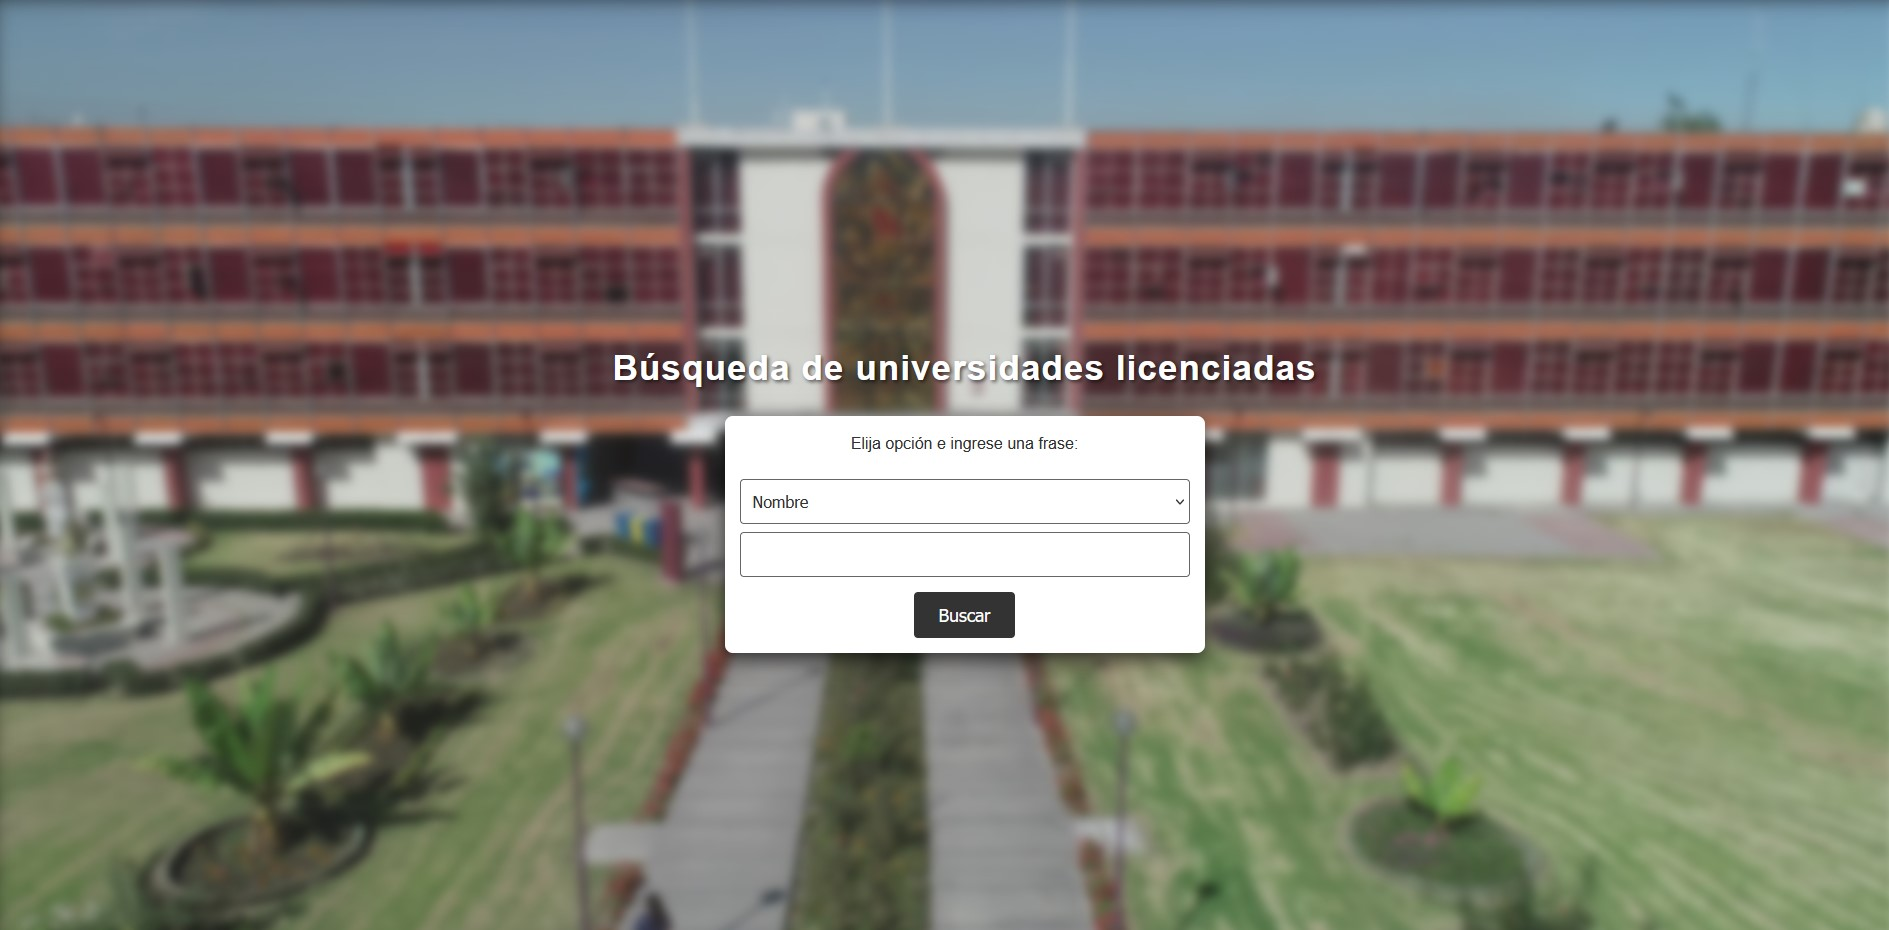
\includegraphics[width=0.8\textwidth]{img1.jpg}
        \caption{SitioWeb01.}
        \label{fig:img1}
    \end{figure}
    
    % Segunda imagen
    \begin{figure}[ht]
        \centering
        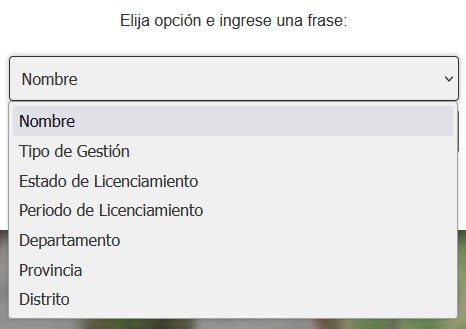
\includegraphics[width=0.4\textwidth]{img2.jpg}
        \caption{SitioWeb02.}
        \label{fig:img2}
    \end{figure}
    
    % Tercera imagen
    \begin{figure}[ht]
        \centering
        
\includegraphics[width=0.8\textwidth]{img3.jpg}
        \caption{Busqueda por Departamento.}
        \label{fig:img3}
    \end{figure}
    
    \newpage
	\section{\textcolor{cyan}{Rúbricas de calificaciones}}
	
	\begin{table}[H]
		\caption{Estudiante \textbf{Auccacusi Conde Brayan Carlos}}
		\setlength{\tabcolsep}{0.5em} % for the horizontal padding
		{\renewcommand{\arraystretch}{1.5}% for the vertical padding
		%\begin{center}
		\begin{tabular}{|p{2.7cm}|p{7cm}|x{1.3cm}|p{1.2cm}|p{1.5cm}|p{1.1cm}|}
			\hline
    		\multicolumn{2}{|c|}{Contenido y demostración} & Puntos & Checklist & Estudiante & Profesor\\
			\hline
			\textbf{1. GitHub} & Hay enlace URL activo del directorio para el  laboratorio hacia su repositorio GitHub con código fuente terminado y fácil de revisar. &2 &X &2 & \\ 
			\hline
			\textbf{2. Commits} &  Hay capturas de pantalla de los commits más importantes con sus explicaciones detalladas. (El profesor puede preguntar para refrendar calificación). &4 &X &4 & \\ 
			\hline 
			\textbf{3. Código fuente} &  Hay porciones de código fuente importantes con numeración y explicaciones detalladas de sus funciones. &2 &X &2 & \\ 
			\hline 
			\textbf{4. Ejecución} & Se incluyen ejecuciones/pruebas del código fuente  explicadas gradualmente. &2 &X &2 & \\ 
			\hline			
			\textbf{5. Pregunta} & Se responde con completitud a la pregunta formulada en la tarea.  (El profesor puede preguntar para refrendar calificación).  &2 &X &2 & \\ 
			\hline	
			\textbf{6. Fechas} & Las fechas de modificación del código fuente estan dentro de los plazos de fecha de entrega establecidos. &2 &X &2 & \\ 
			\hline 
			\textbf{7. Ortografía} & El documento no muestra errores ortográficos. &2 &X &2 & \\ 
			\hline 
			\textbf{8. Madurez} & El Informe muestra de manera general una evolución de la madurez del código fuente,  explicaciones puntuales pero precisas y un acabado impecable.   (El profesor puede preguntar para refrendar calificación).  &4 &X &2 &\\
			\hline
			\multicolumn{2}{|c|}{\textbf{Total}} &20 & &18 & \\ 
			\hline
		\end{tabular}
		%\end{center}
		%\label{tab:multicol}
		}
	\end{table}

	\begin{table}[H]
		\caption{Estudiante \textbf{Palma Apaza Santiago Enrique}}
		\setlength{\tabcolsep}{0.5em} % for the horizontal padding
		{\renewcommand{\arraystretch}{1.5}% for the vertical padding
		%\begin{center}
		\begin{tabular}{|p{2.7cm}|p{7cm}|x{1.3cm}|p{1.2cm}|p{1.5cm}|p{1.1cm}|}
			\hline
    		\multicolumn{2}{|c|}{Contenido y demostración} & Puntos & Checklist & Estudiante & Profesor\\
			\hline
			\textbf{1. GitHub} & Hay enlace URL activo del directorio para el  laboratorio hacia su repositorio GitHub con código fuente terminado y fácil de revisar. &2 &X &2 & \\ 
			\hline
			\textbf{2. Commits} &  Hay capturas de pantalla de los commits más importantes con sus explicaciones detalladas. (El profesor puede preguntar para refrendar calificación). &4 &X &4 & \\ 
			\hline 
			\textbf{3. Código fuente} &  Hay porciones de código fuente importantes con numeración y explicaciones detalladas de sus funciones. &2 &X &2 & \\ 
			\hline 
			\textbf{4. Ejecución} & Se incluyen ejecuciones/pruebas del código fuente  explicadas gradualmente. &2 &X &2 & \\ 
			\hline			
			\textbf{5. Pregunta} & Se responde con completitud a la pregunta formulada en la tarea.  (El profesor puede preguntar para refrendar calificación).  &2 &X &2 & \\ 
			\hline	
			\textbf{6. Fechas} & Las fechas de modificación del código fuente estan dentro de los plazos de fecha de entrega establecidos. &2 &X &2 & \\ 
			\hline 
			\textbf{7. Ortografía} & El documento no muestra errores ortográficos. &2 &X &2 & \\ 
			\hline 
			\textbf{8. Madurez} & El Informe muestra de manera general una evolución de la madurez del código fuente,  explicaciones puntuales pero precisas y un acabado impecable.   (El profesor puede preguntar para refrendar calificación).  &4 &X &2 &\\
			\hline
			\multicolumn{2}{|c|}{\textbf{Total}} &20 & &18 & \\ 
			\hline
		\end{tabular}
		%\end{center}
		%\label{tab:multicol}
		}
	\end{table}    

	\begin{table}[H]
		\caption{Estudiante \textbf{Pamo Condori Benjamin Andre}}
		\setlength{\tabcolsep}{0.5em} % for the horizontal padding
		{\renewcommand{\arraystretch}{1.5}% for the vertical padding
		%\begin{center}
		\begin{tabular}{|p{2.7cm}|p{7cm}|x{1.3cm}|p{1.2cm}|p{1.5cm}|p{1.1cm}|}
			\hline
    		\multicolumn{2}{|c|}{Contenido y demostración} & Puntos & Checklist & Estudiante & Profesor\\
			\hline
			\textbf{1. GitHub} & Hay enlace URL activo del directorio para el  laboratorio hacia su repositorio GitHub con código fuente terminado y fácil de revisar. &2 &X &2 & \\ 
			\hline
			\textbf{2. Commits} &  Hay capturas de pantalla de los commits más importantes con sus explicaciones detalladas. (El profesor puede preguntar para refrendar calificación). &4 &X &4 & \\ 
			\hline 
			\textbf{3. Código fuente} &  Hay porciones de código fuente importantes con numeración y explicaciones detalladas de sus funciones. &2 &X &2 & \\ 
			\hline 
			\textbf{4. Ejecución} & Se incluyen ejecuciones/pruebas del código fuente  explicadas gradualmente. &2 &X &2 & \\ 
			\hline			
			\textbf{5. Pregunta} & Se responde con completitud a la pregunta formulada en la tarea.  (El profesor puede preguntar para refrendar calificación).  &2 &X &2 & \\ 
			\hline	
			\textbf{6. Fechas} & Las fechas de modificación del código fuente estan dentro de los plazos de fecha de entrega establecidos. &2 &X &2 & \\ 
			\hline 
			\textbf{7. Ortografía} & El documento no muestra errores ortográficos. &2 &X &2 & \\ 
			\hline 
			\textbf{8. Madurez} & El Informe muestra de manera general una evolución de la madurez del código fuente,  explicaciones puntuales pero precisas y un acabado impecable.   (El profesor puede preguntar para refrendar calificación).  &4 &X &2 &\\
			\hline
			\multicolumn{2}{|c|}{\textbf{Total}} &20 & &18 & \\ 
			\hline
		\end{tabular}
		%\end{center}
		%\label{tab:multicol}
		}
	\end{table}    

	\begin{table}[H]
		\caption{Estudiante \textbf{Huaynacho Mango Jerry Anderson}}
		\setlength{\tabcolsep}{0.5em} % for the horizontal padding
		{\renewcommand{\arraystretch}{1.5}% for the vertical padding
		%\begin{center}
		\begin{tabular}{|p{2.7cm}|p{7cm}|x{1.3cm}|p{1.2cm}|p{1.5cm}|p{1.1cm}|}
			\hline
    		\multicolumn{2}{|c|}{Contenido y demostración} & Puntos & Checklist & Estudiante & Profesor\\
			\hline
			\textbf{1. GitHub} & Hay enlace URL activo del directorio para el  laboratorio hacia su repositorio GitHub con código fuente terminado y fácil de revisar. &2 &X &2 & \\ 
			\hline
			\textbf{2. Commits} &  Hay capturas de pantalla de los commits más importantes con sus explicaciones detalladas. (El profesor puede preguntar para refrendar calificación). &4 &X &4 & \\ 
			\hline 
			\textbf{3. Código fuente} &  Hay porciones de código fuente importantes con numeración y explicaciones detalladas de sus funciones. &2 &X &2 & \\ 
			\hline 
			\textbf{4. Ejecución} & Se incluyen ejecuciones/pruebas del código fuente  explicadas gradualmente. &2 &X &2 & \\ 
			\hline			
			\textbf{5. Pregunta} & Se responde con completitud a la pregunta formulada en la tarea.  (El profesor puede preguntar para refrendar calificación).  &2 &X &2 & \\ 
			\hline	
			\textbf{6. Fechas} & Las fechas de modificación del código fuente estan dentro de los plazos de fecha de entrega establecidos. &2 &X &2 & \\ 
			\hline 
			\textbf{7. Ortografía} & El documento no muestra errores ortográficos. &2 &X &2 & \\ 
			\hline 
			\textbf{8. Madurez} & El Informe muestra de manera general una evolución de la madurez del código fuente,  explicaciones puntuales pero precisas y un acabado impecable.   (El profesor puede preguntar para refrendar calificación).  &4 &X &2 &\\
			\hline
			\multicolumn{2}{|c|}{\textbf{Total}} &20 & &18 & \\ 
			\hline
		\end{tabular}
		%\end{center}
		%\label{tab:multicol}
		}
	\end{table}    
	
\clearpage

\section{Referencias}
\begin{itemize}			
	\item \url{https://www.w3schools.com/java/default.asp}
	\item \url{https://www.geeksforgeeks.org/insertion-sort/}
	\item \url{https://www.w3schools.com/java/default.asp}
	\item \url{https://www.geeksforgeeks.org/insertion-sort/}
	\item \url{https://docs.github.com/en/github/collaborating-with-issues-and-pull-requests/about-issues}
	\item \url{https://www.git-scm.com/book/en/v2/Getting-Started-About-Version-Control}
	\item \url{https://www.atlassian.com/git/tutorials/comparing-workflows}
	\item \url{https://www.educative.io/edpresso/what-are-pull-requests-in-git}
	\item \url{https://www.gitkraken.com/learn/git/tutorials/git-merge-conflict}
	\item \url{https://dev.to/rammyblog/how-to-merge-and-resolve-conflicts-in-git-2dgp}
	\item \url{https://www.turing.com/kb/what-is-git-and-why-is-it-important}
	\item \url{https://stackabuse.com/understanding-and-resolving-git-merge-conflicts/}
	\item \url{https://www.learngitbranching.js.org/}
	\item \url{https://www.geeksforgeeks.org/git-merge-conflict/}
	\item \url{https://opensource.com/article/19/11/why-use-git}
\end{itemize}
	
%\clearpage
%\bibliographystyle{apalike}
%\bibliographystyle{IEEEtranN}
%\bibliography{bibliography}
			
\end{document}